%Monthly report for the PuMA fuel meter project
%Created by Doug Keller

\documentclass[12pt,a4paper]{article}

\usepackage{fancyhdr,url,graphicx,caption,tabu,varwidth}
\usepackage[a4paper, top = 1in, bottom = 1in, left = .75in, right = .75in]{geometry}
\renewcommand{\familydefault}{\sfdefault}
\fancyfoot{}
\fancyhead{}
\pagestyle{fancy}

\fancyhead[L]{
\includegraphics[height = 32pt]{../Logos/acep.pdf}\\}
\fancyhead[R]{\includegraphics[height = 24pt]{../Logos/uaf_blue_hor.pdf}\\}
\fancyfoot[L]{\scriptsize{Alaska}}
\renewcommand{\headrulewidth}{0pt}

\setlength{\parindent}{0pt}
\setlength{\fboxrule}{.8pt}
\usepackage[font = footnotesize, textfont=it, labelfont= bf]{caption}

\newcommand{\totalusage}{2.845}
\newcommand{\fuelperday}{0.092}
\newcommand{\fuelprice}{3}
\newcommand{\totalcost}{8.53}
\newcommand{\fuelcostperday}{0.28}
\newcommand{\neighborusage}{3.287}
\newcommand{\percentusage}{13.45}
\newcommand{\moreless}{less}
\newcommand{\reportmonth}{May}
\newcommand{\reportyear}{2019}
\newcommand{\progress}{65.63}
\newcommand{\progressmoreless}{less}


\begin{document}

\begin{center}
\textbf{\Huge{\\Monthly Fuel Usage Report}}
\end{center}

\begin{center}
	\fbox{
		\begin{varwidth}{.8\textwidth}
			This month you consumed {\percentusage}\% {\moreless} than your neighbors.
		\end{varwidth}
	}
\end{center}

\vspace{12pt}

\begin{tabu}{X[m,c]|X[m,c]}

	\includegraphics[width = 3in]{monthly_fuel_usage.png}
	
	&
	
	\underline{{\reportmonth} {\reportyear} Fuel Usage:}
	
		\begin{description}
		
			\centering
			
			\item Total Usage (gal): {\totalusage}
			
			\item Price of Fuel (\$/gal): {\fuelprice}
			
			\item Total Cost (\$): {\totalcost}
			
		\end{description}
	
	
\end{tabu}

\vspace{12pt}
\rule{\textwidth}{1pt}
\vspace{12pt}

\begin{tabu}{X[m,c]X[m,c]}

	\underline{This month:}
	
	\begin{itemize}
	
	\item Your average fuel consumption was {\fuelperday} gallons per day.
	\item Your average fuel cost was \${\fuelcostperday} per day

	\end{itemize}

	&
	
	\includegraphics[width = 3in]{monthly_polar_plot.png}

\end{tabu}

\vspace{12pt}
\rule{\textwidth}{1pt}
\vspace{12pt}

\underline{Track Your Progress:}\\

You used {\progress}\% {\progressmoreless} this month than last month.\\

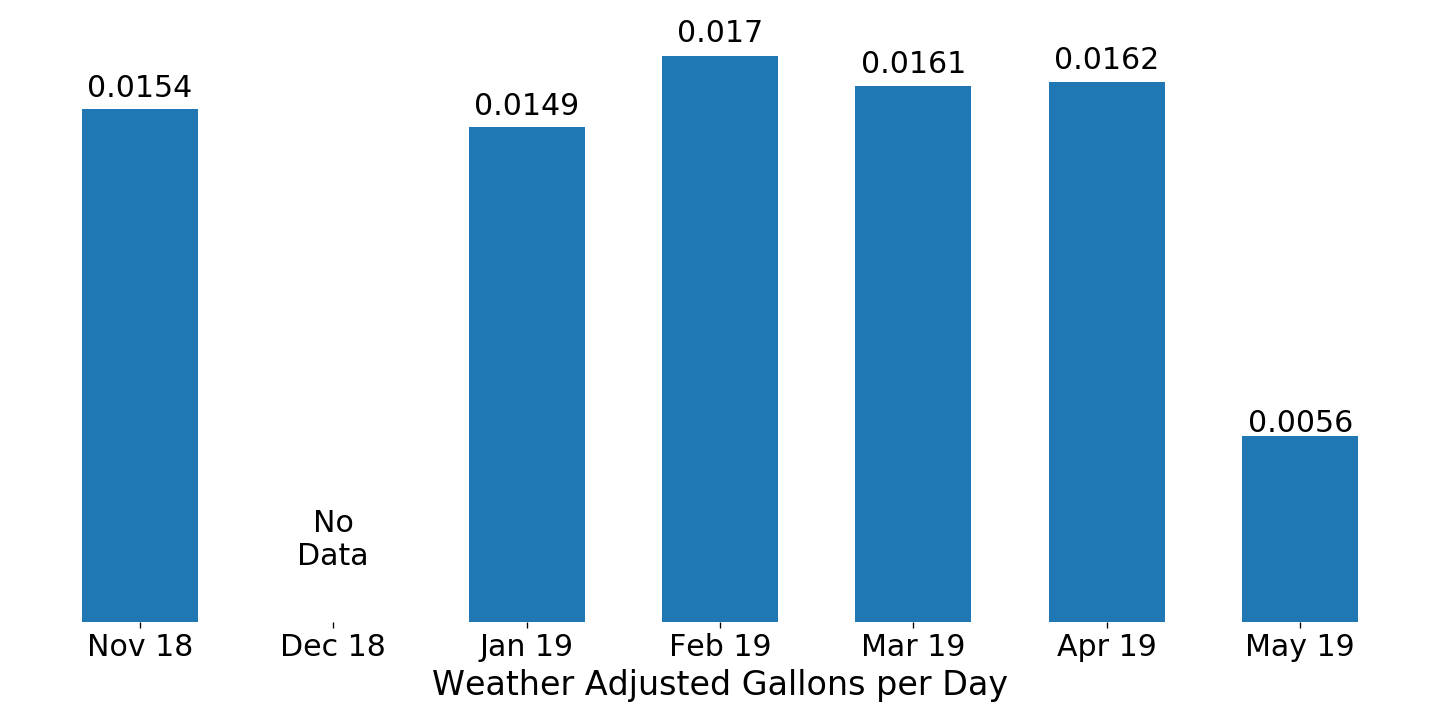
\includegraphics[width = 6in]{monthly_track_your_progress.png}

\vspace{12pt}
\rule{\textwidth}{1pt}
\vspace{12pt}

\section*{Tips}

%\begin{figure}[h]
%\captionsetup{justification = centering, margin = 1in}
%\centering
%\includegraphics[width = 480pt]{.png}
%\caption{\label{gantt}}
%\end{figure}

\end{document}